\documentclass[parskip=full]{scrreprt}
% Paket um vordefinierte Texte (z.B. "Inhaltsverzeichnis") auf Deutsch zu übersetzen
\usepackage[ngerman]{babel}

% Paket um Schriftarten festzulegen (für XeLaTeX)
\usepackage{fontspec}

% Schriftart festlegen
\usepackage{lmodern}
\renewcommand{\familydefault}{\sfdefault}

\setmonofont[]{Hack}

% Farben
\usepackage{xcolor}
\definecolor{TeLicolor}{RGB}{90, 95, 110}
\definecolor{plusGreen}{RGB}{0, 150, 0}
\definecolor{minusRed}{RGB}{200, 0, 0}
\definecolor{boxBG}{RGB}{230, 230, 230}
\definecolor{boxFrame}{RGB}{50, 50, 50}

% Für Untertitel
\usepackage{caption}
\usepackage{subcaption}

% Paket zur Erstellung von Zeichnungen
\usepackage{tikz}
\usetikzlibrary{positioning}

% Für SI Schreibweise
\usepackage{siunitx}

% Mathe
\usepackage{amsmath}

% Paket um Grafiken (JPG, PNG, PDF) einzubinden
\usepackage{graphicx}
\graphicspath{{pictures/}}

% Pakete für Tabellenlayout
\usepackage{booktabs}
\usepackage{tabularx}

% Paket für Syntaxhighlighting für inline code
\usepackage[minted]{tcolorbox}
\usemintedstyle{manni}
\tcbuselibrary{listingsutf8}
\newtcolorbox{codeblock}[1][]{%
  colback=boxBG
  colframe=boxFrame
  boxrule=0.4pt,        % Rahmenstärke
  arc=2mm,              % abgerundete Ecken
  outer arc=2mm,
  boxsep=2pt,           % Innenabstand
  left=2pt, right=2pt, top=2pt, bottom=2pt,
  listing only,
  minted options={fontsize=\small, breaklines, #1}
}

\tcbuselibrary{skins, breakable}
\newtcolorbox{imgbox}[1][]{%
  enhanced,
  colback=boxBG,
  colframe=boxFrame,
  boxrule=0.4pt,
  arc=2mm,
  outer arc=2mm,
  boxsep=3pt,
  left=3pt, right=3pt, top=3pt, bottom=3pt,
  #1
}

% Befehl für einzelne, farbige interne Links
\newcommand{\TeLi}[1]{%
  \begingroup
    \hypersetup{linkcolor=TeLicolor}%
    \ref{#1}%
  \endgroup
}

\newcommand{\hTeLi}[2]{%
  \begingroup
    \hypersetup{linkcolor=TeLicolor}%
    \hyperref[#1]{#2}%
  \endgroup
}

\newcommand{\aTeLi}[1]{%
  \begingroup
    \hypersetup{linkcolor=TeLicolor}%
    \autoref{#1}%
  \endgroup
}

% Paket für Zeilenabstand
\usepackage{setspace}

% Paket für Hyperlinks
\usepackage[
  colorlinks=true,
  linkcolor=black,      % For internal links (like table of contents)
  citecolor=black,      % For citations
  urlcolor=blue         % For URLs
]{hyperref}

% Paket für korrekte Anführungszeichen
\usepackage{csquotes}

% Paket für selbst definierte Kopf- und Fusszeilen
\usepackage{scrlayer-scrpage}

% Pakte für Zitate und Bibliografie
\usepackage[style=ieee, citestyle=numeric-comp]{biblatex}
\addbibresource{literature.bib}

% Paket zum Erzeugen von Platzhaltertext
\usepackage{blindtext}

% Schmale Seitenränder festlegen
\KOMAoption{DIV}{15}

% Variablen
\newcommand{\maTitle}{Autonom durch die Lüfte: Die Integration von Gestenerkennung in die Navigation eines Mini-Hubschraubers}
\newcommand{\chapOne}{Einleitung}
\newcommand{\chapTwo}{Theorie}
\newcommand{\chapThree}{Methode}
\newcommand{\chapFour}{Ergebnisse}
\newcommand{\chapFive}{Diskussion und Fazit}

% Für Code im Fliesstext
\newcommand{\bodyCode}[1]{\texttt{\small #1}}

% Für Code der alleine steht
% Usage: \codefile[filename]{caption}{label}
\newcommand{\codefile}[3][]{%
    \begin{minipage}{\linewidth}
        \vspace{1ex}
        \captionsetup{type=listing,labelformat=empty}
        \caption*{\large{\textbf{#2}}}
        \label{#3}
        \vspace{-1ex}
        \begin{codeblock}[#1]
            \inputminted[
                fontsize=\small,
                breaklines=true,
                linenos=false
            ]{python}{code_snippets/#1}
        \end{codeblock}
    \end{minipage}
}

% Für Mathe im Fliesstext
\newcommand{\inlinemath}[1]{\(#1\)}

% Für Math
\newcommand{\cp}{\textcolor{plusGreen}{\texttt{+}}}
\newcommand{\cm}{\textcolor{minusRed}{\texttt{-}}}

% Für Tech-Wörter
\newcommand{\techWord}[1]{\textit{#1}}

% Text auf Titelseite festlegen
\subject{Maturaarbeit}
\title{\maTitle}
\author{Nelio Gautschi\vspace{1cm}\\
Betreut durch \\
Stefan Rothe}
\publishers{
\includegraphics{logo}\vspace{1cm}\\
Gymnasium Kirchenfeld\\
Abteilung GH}

% selbst definierte Kopf- und Fusszeile
\lohead{Maturaarbeit}

%\rohead{\theauthor}
\cofoot{\thepage}

% Zeilenabstand festlegen
\singlespacing %\doublespacing \onehalfspacing

% Trennlinie für Kopfzeile
\KOMAoption{headsepline}{off}

% Trennlinie für Fusszeile
\KOMAoption{footsepline}{on}

% ANFANG DOKUMENT -----------------------------------
\begin{document}

% erstelle Titel
\maketitle

\chapter*{Danksagung}
\label{cha:ack}

\begingroup
\fontsize{12pt}{14pt}\selectfont

Ich möchte zuallererst Stefan Rothe für sein Vertrauen in mich und meine Ideen danken.  
Auch für sein Interesse und die Förderung meiner Begeisterung für das Programmieren bin ich ihm dankbar.

Ebenso danke ich Andreas Gautschi für sein professionelles Feedback und seine inspirierenden Anregungen sowie fürs Entfachen der Begeisterung am Pogrammieren.

Besonderer Dank gilt Inga Eickemeier Gautschi, die jedes Wort überprüft hat und sicherstellte, dass ich diese Arbeit im vorgegebenen zeitlichen Rahmen beenden konnte.

Herzlich danke ich Maxime Klinkert für ihre Rücksichtnahme, ihr Verständnis und ihre Unterstützung – trotz der vielen Nächte, in denen der Computer unser Schlafzimmer beleuchtete.

Schliesslich gilt mein Dank Rufus Spyra für seine ermunternden Worte und Ideen in nächtlichen Krisensituationen.

\endgroup

\tableofcontents
\clearpage

\begingroup
    \let\clearpage\relax
    \listoffigures
    \listoftables
\endgroup

\chapter{\chapOne}
\label{cha:chapter1} % Label for hyperlink

% Start font-size
\begingroup
\fontsize{12pt}{14pt}\selectfont

\section{Einführung ins Thema}
Gestenerkennung und Gestensteuerung haben sich in den letzten Jahren von Nischenanwendungen im Gaming-Bereich wie beispielsweise der Kinect-Plattform~\cite{Wiki:Kinect} zu vielseitigen Steuerungsmöglichkeiten für virtuelle und reale Umgebungen entwickelt~\cite{RG:GestureRecognition}.
Ihre Wurzeln liegen teilweise in der Analyse der Gebärdensprache, reichen jedoch letztlich bis zu den Anfängen menschlicher Kommunikation zurück.\cite{Wiki:Gestenerkennung}\cite{RG:Gesten}
Gesten stellen einen festen und wesentlichen Bestandteil der nonverbalen Verständigung dar und bilden somit eine natürliche Grundlage für intuitive Interaktionsformen zwischen Mensch und Maschine.\cite[10]{Hobmair:Psy}

Parallel dazu gewinnt die autonome Steuerung technischer Systeme zunehmend an Bedeutung.
Fahrzeuge, die mit modernen Fahrassistenzsystemen ausgestattet sind, können heute vom Spurhalten bis zum automatischen Parkieren fast alles selbstständig ausführen.
Doch nicht nur im Strassenverkehr, auch in der Luft- und Schifffahrt werden Prozesse automatisiert, um Effizienz und Sicherheit zu erhöhen und menschliche Fehler zu minimieren.
Trotz dieser Entwicklungen bleibt der Mensch ein zentraler Bestandteil des Kontrollsystems: Er kann jederzeit in den automatisierten Ablauf eingreifen und die Steuerung übernehmen.\cite{Wiki:aupi}

Noch rasanter schreitet die Entwicklung im Bereich der virtuellen und erweiterten Realität (VR und AR) voran~\cite{SD:VR}.
Hier ermöglichen innovative Interaktionskonzepte eine immer natürlichere, präzisere und intuitivere Steuerung digitaler Umgebungen.
Ein beeindruckendes Bespiel ist dabei die \textit{Apple Vision Pro}, eine VR-Brille, die im Jahr 2023 auf den Märkten erschienen ist.
Das Gerät verfolgt die Bewegung der Augen und verwendet diese als Gestensteuerung und erlaubt es durch Zusammenführen von Daumen und Zeigefinger Objekte auf dem virtuellen Bildschirm auszuwählen.\cite{apl:vision}

Auch in der Robotik eröffnen Gestensteuerungssysteme neue Perspektiven: Sie erlauben eine direkte, beinahe natürliche Kommunikation mit semi-autonomen oder autonomen Geräten, etwa bei der Navigation von Drohnen oder mobilen Robotern.
So können beispielsweise Bergungsarbeiten oder Minenräumungen künftig aus sicherer Entfernung durchgeführt werden, ohne dabei Menschen unnötigen Gefahren auszusetzen.

\section{Zielsetzung der Arbeit}
Das Ziel dieser Arbeit ist es, die Konzepte der Gestenerkennung sowie deren Einsatzmöglichkeiten zur Steuerung virtueller Systeme zu veranschaulichen.
Als Grundlage dient dabei ein ähnliches Projekt, welches ein neurales Netzwerk zur Erkennung von Handpositionen implementiert, um eine Steuerungsalternative zu traditionellen Kontrollern zu bieten.
Die Position der Hand wird von einer Kamera erfasst und von einem Computer ausgewertet.
Dieser sendet Steuerbefehle anhand der berechneten Daten an einer Renndrohne.\cite{arxiv:OmniRace}

Um den Aufwand in einem realistischen Rahmen zu halten, wird in dieser Arbeit nicht auf eine direkte Erkennung der Fingerpositionen gesetzt.
Stattdessen kommen vier ArUco-Marker zum Einsatz, die auf der Steuerhand befestigt werden.
Dies soll eine präzise Erkennung der Handausrichtung ermöglichen, indem Flächen, Positionen und Distanzen der Marker berechnet und verglichen werden.
Anschliessend wird mit den in \hTeLi{sec:cf}{Kapiteln~\ref{sec:cf}} und \hTeLi{sec:crpa}{\ref{sec:crpa}} beschriebenen Hardware-Komponenten eine Drohne gesteuert.

In diesem Projekt werden zwei Ansätze getestet, die sich in der Platzierung der Marker unterscheiden.
Der erste Ansatz sieht die Marker in einem Rechteck angeordnet vor, wobei ausschliesslich die Handfläche als Bereich für die Marker dient.
Der zweite Versuch setzt hingegen drei von vier Markern auf den Fingerspitzen vorraus.
Der vierte Marker wird auf dem Handgelenk platziert und markiert für die Kamera den Referenzpunkt der Hand.

Die unterschiedliche Platzierung der Marker soll zeigen, inwieweit die Einbeziehung der Finger die Erkennungsgenauigkeit und Steuerung beeinflusst.

\subsection{Fragestellung}
Wie beeinflusst die Platzierung von ArUco-Markern auf der Hand die Genauigkeit und Zuverlässigkeit einer gestenbasierten Steuerung einer Nano-Drohne?  
Lässt sich durch die Einbeziehung der Finger in die Markeranordnung eine präzisere Erkennung der Handausrichtung und damit eine stabilere Steuerung erreichen?

\subsection{Abgrenzung (ausgeschlossene Faktoren)}
Im Rahmen dieses Projekts werden externe Einflussfaktoren bewusst ausgeklammert beziehungsweise nicht im Detail untersucht.
Dazu gehören insbesondere:
\begin{itemize}
  \item \textbf{Licht- und Belichtungsverhältnisse:} Es wird von konstanten, guten Lichtverhältnissen ausgegangen.
  \item \textbf{Wind- und Luftströmungen:} Das System wird ausschliesslich in einer windstillen Indoor-Umgebung getestet.
  \item \textbf{Funkstörungen:} Potenzielle Interferenzen durch andere Funkgeräte oder Netzwerke werden nicht berücksichtigt.
  \item \textbf{Komplexe Handgesten:} Es wird davon ausgegangen, dass die ArUco-Tags jederzeit für die Kamera sichtbar bleiben.
  \item \textbf{Entfernung zur Kamera:} Die Entfernung zwischen der Kamera und der Hand in neutraler Position soll idealerweise so wenig wie möglich variieren.
\end{itemize}

\subsection{Hypothese}
Eine Markeranordnung, welche auch die Finger einbezieht, ermöglicht eine präzisere Bestimmung der Handausrichtung und führt somit zu einer zuverlässigeren und stabileren Steuerung der Drohne als eine ausschliesslich auf der Handfläche platzierte Markeranordnung.

% End font-size
\endgroup
\chapter{\chapTwo}
\label{sec:kapitel2} % Label for hyperlink

% Start font-size
\begingroup
\fontsize{12pt}{14pt}\selectfont

\section{OpenCV}
\label{sec:ocv} % Label for hyperlink
OpenCV steht für \enquote{Open Source Computer Vision Library} und ist eine der umfangreichsten Bibliotheken für die Echtzeit-Verarbeitung visueller Daten. Das \enquote{Open} im Namen weist darauf hin, dass es sich um ein Open-Source-Projekt handelt. Der Quelltext ist also öffentlich zugänglich und darf unter Einhaltung der Lizenzbedingungen verändert und kostenfrei verwendet werden. OpenCV stellt mehrere sogenannte \textit{Dictionaries} (im Folgenden als \enquote{Bibliotheken} bezeichnet) bereit, die über 2500 Algorithmen beinhalten.
Die Bibliothek OpenCV wurde in C\texttt{++} implementiert, um eine hohe Rechenleistung, Plattformunabhängigkeit und eine modulare Struktur zu gewährleisten. Auf Basis des C\texttt{++}-Kerns sind später Schnittstellen für Python, Java und andere Sprachen entstanden, die die Nutzung der Bibliothek erleichtern \cite{ocv:org}\footnote{\url{opencv.org/about}}.

\subsection{Einsatzbereiche}
OpenCV findet Anwendung in vielen Bereichen der Bildverarbeitung. Die Bibliothek eignet sich insbesondere für Aufgaben, die eine effiziente Verarbeitung von Bildern und Videos in Echtzeit erfordern. 
Im Folgenden sind einige typische Beispiele aufgelistet \cite{Wiki:ocv}

\begin{minipage}{0.55\textwidth}
    \begin{enumerate}
        \item Automatisierte Gesichtserkennung
        \item Gestenerkennung
        \item Bewegungsanalyse
        \item Objektidentifizierung
    \end{enumerate}
\end{minipage}
\hfill
\begin{minipage}{0.4\textwidth}
    \begin{figure}[H]
        \centering
            
\includegraphics[width=0.5\textwidth]{ocv_logo.pdf}
        \caption{Logo von OpenCV \cite{ocv:org}.}
            \label{fig:ocv_logo}
    \end{figure}
\end{minipage}

Abgesehen von diesen klassischen Anwendungsfeldern wird OpenCV auch zunehmend in Forschungsprojekten genutzt, beispielsweise zur Gesten- oder Marker-basierten Steuerung von Robotiksystemen, wie sie im Rahmen dieser Arbeit zum Einsatz kommt. \cite{sse:foodDel}

\subsection{Module}

\section{ArUco-Marker}
Ein ArUco-Marker (wie in \autoref{fig:marker0} dargestellt) ist ein quadratischer Referenzmarker, der zur Positions- und Orientierungserkennung in Bildern bzw. Kamerasystemen zum Einsatz kommt. Referenzmarker (auch Passermarken) werden ursprünglich in automatisierten Fertigungsverfahren von elektronischen Bauelementen wie beispielsweise Hauptplatinen verwendet. Sie dienen als optische Referenzpunkte für die Maschinen, die am Fertigungsprozess beteiligt sind. Dadurch erhöhen sie die Präzision und reduzieren Kurzschlüsse \cite{Wiki:Passermarke}.
Es gibt Referenzmarker in verschiedenen Grössen, Farbschemen und Formen, abhängig von ihrem Einsatzgebiet. Für diese Arbeit werden aus folgenden Gründen quadratische benutzt:

\begin{itemize}
    \item Die Erkennung der Marker erfolgt schnell und effizient, was bei Echtzeitsteuerung vorteilhaft ist.
    \item Quadratische Marker werden häufig gebraucht und sind daher ausführlicher dokumentiert als andere.
    \item Sie sind relativ einfach einzusetzen.
\end{itemize}

ArUco-basierte Marker zählen zu den verlässlichsten, vor allem seit \hyperref[sec:ocv]{OpenCV} ein Submodul zur Implementierung dieser Marker hinzugefügt hat \cite{IJ:fiducial}.

\begin{figure}[H]
    \centering
        
\includegraphics[width=0.3\textwidth]{aruco.pdf}
    \caption{ArUco-Marker mit ID 0. Generiert von \cite{chev:arucogen}}.
        \label{fig:marker0}
\end{figure}

\subsection{Funktionsweise}
Das Schwarzweiss-Schema von ArUco-Markern erinnert an das eines QR-Codes. Während beide einem ähnlichen Zweck dienen, nämlich der visuellen Identifizierung von Objekten, ist ihr geometrischer Aufbau grundverschieden \cite{ten:qrcode}.
Die Fabrikation von QR-Codes beruht auf drei Hauptbestandteilen:

\begin{enumerate}
    \item Menge der codierten Information.
    \item Modus, in dem die Daten codiert wurden.
    \item Stärke der Fehlerkorrekturfunktion.
\end{enumerate}

Der entscheidende Unterschied zwischen dieser Funktionsweise und der von ArUco-Markern ist der Informationgehalt. Bei ArUco-Markern existiert dieser nicht. Sie sind nicht eine binäre Übersetzung einer vordefinierten Eingabe, sondern sind in nummerierten Bibliotheken angelegt und besitzen keine versteckte Botschaft. Es gibt keinen Algorithmus, der Klartext in einen ArUco-Marker übersetzt. Dieses Konzept hat seine Vor- und Nachteile. Einerseits erhöht es die Geschwindigkeit der Identifizierung, andererseits limitiert es die Gesamtmenge aller Marker. Diese Bedingungen sind jedoch ideal für dieses Projekt, da nur wenige verschiedene Marker benötigt werden und Effizienz gefragt ist. 
Um einen gesuchten Marker in den Bibliotheken zu finden, braucht man den Namen der Bibliothek und die ID des Markers. Der Name der Bibliothek legt die Grösse der Matrix und somit Komplexität des Markers fest sowie die Anzahl möglicher Marker.

\begin{table}[H]
    \centering
    \begin{tabular}{lcc}
        \toprule
        \textbf{Bibliothek} & \textbf{Datenbits} & \textbf{Markeranzahl} \\
        \midrule
        DICT\_4X4\_50 & 16 & 50 \\
        DICT\_4X4\_100 & 16 & 100 \\
        DICT\_5X5\_50 & 25 & 50 \\
        \bottomrule
    \end{tabular}
    \caption{Eigenschaften ausgewählter ArUco-Dictionaries.}
        \label{tab:aruco_dicts}
\end{table}

In der Tabelle \autoref{tab:aruco_dicts} sind drei Bibliotheken und deren Eigenschaften dargestellt. Es ist zu beachten, dass alle Marker der Bibliothek \bodyCode{DICT\_4X4\_50} auch in \bodyCode{DICT\_4X4\_100} vorhanden sind, da die größere Bibliothek alle IDs der kleineren umfasst. Für dieses Projekt wird die Bibliothek \bodyCode{DICT\_4X4\_50} verwendet, weil es die geometrisch unkomplizierteste Bibliothek ist, die OpenCV unterstützt. Das ist insofern wichtig, weil die Markern letztendlich unter Winkeln bis zu 45° erkennbar sein sollen. Da weitaus weniger als fünfzig Marker benötigt werden, reicht die \bodyCode{\_50} Bibliothek aus.

\section{Mathematische Grundlagen}

\subsection{Flächenberechnung mit gaussschen Trapezformel}

\section{Crazyflie 2.0}

\subsection{cflib}

\section{Crazyradio PA}

% End font-size
\endgroup
\chapter{\chapThree}
\label{cha:chapter3} % Label for hyperlink

% Start font-size
\begingroup
\fontsize{12pt}{14pt}\selectfont

In diesem Kapitel wird beschrieben, wie die in \hTeLi{cha:chapter2}{Kapitel~\ref{cha:chapter2}} vorgestellten theoretischen Grundlagen praktisch umgesetzt werden.
Ziel ist es, eine Gestensteuerung der Crazyflie 2.0 mithilfe von ArUco-Markern zu realisieren.
Um dieses Ziel zu erreichen, wurde eine zwei Methoden entwickelt, die sowohl die Erkennung und Analyse von Handbewegungen als auch die Steuerung der Drohne umfasst.

\section{Vorgehensweise}

Beide Methoden umfassen die selben Prozessschritte, die von der Erfassung visueller Daten über deren mathematische Verarbeitung bis hin zur Umsetzung in Steuerbefehle für die Drohne reichen.
Der ausschlaggebende Unterschied ist dabei die Platzierung der Marker auf der Hand (mehr dazu in \hTeLi{sec:diff_meth}{Kapitel~\ref{sec:diff_meth}}).
Innerhalb beider Methoden werden folgende Schritte durchgeführt:

\begin{enumerate}
    \item \textbf{Erfassen der Handbewegung:}
    \begin{itemize}
        \item Kameraerfassung der ArUco-Marker auf der Hand.
        \item Verarbeitung der Bilder mit OpenCV.
        \item Extraktion der Markerpositionen und Eckpunkte.
    \end{itemize}
    \item \textbf{Datenverarbeitung und Interpretation:}
    \begin{itemize}
        \item Flächenberechnung jedes Markers mittels Gausscher Trapezformel.
        \item Einmaliges Kalibrieren der Marker.
        \item Bestimmung der Ausrichtung der Handfläche.
    \end{itemize}
    \item \textbf{Steuerung der Crazyflie:}
    \begin{itemize}
        \item Übersetzung der Handausrichtung in Steuerargumente.
        \item Verwendung dieser Argumente in den CFLib-Funktionen.
        \item Übertragung der Befehle über das Crazyradio PA via CRTP.
    \end{itemize}
\end{enumerate}

\section{Unterschiede der Lösungsansätze}
\label{sec:diff_meth}

Wie bereits erwähnt, unterscheiden sich die Methoden in der Platzierung der ArUco-Marker auf der Hand.
Beide Methoden verwenden genau vier Marker, welche die IDs 1 bis 4 darstellen.

\subsection{Methode 1}
In Methode~1 werden die Marker in einem Rechteck platziert.
Als Referenzpunkte dienen dazu die Fingergrundgelenke (\textit{FFG}) und das Handgelenk (\textit{HG}) der Hand:

\begin{itemize}
    \item Marker \bodyCode{ID=1} wird auf das \textit{FGG} des kleinen Fingers geklebt.
    \item Marker \bodyCode{ID=2} wird auf das \textit{FGG} des Indexfingers geklebt.
    \item Marker \bodyCode{ID=3} wird auf die rechte Seite des \textit{HG}s geklebt.
    \item Marker \bodyCode{ID=4} wird auf die linke Seite des \textit{HG}s geklebt.
\end{itemize}

Die Breite des Markerbereichs ist hier als Distanz zwischen den Mittelpunkten der ArUco-Marker mit den IDs 1 und 2 definiert.
Die Höhe ist mit der Entfernung der Mittelpunkte zwischen Marker \bodyCode{ID=1} und \bodyCode{ID=4} gleichzusetzen.

\subsection{Methode 2}
Im Gegensatz zur Methode~1 werden bei Methode~2 die Finger als Teil der Hand mitverwendet.
Markern mit \bodyCode{ID=1} soll auf der Spitze des kleinen Fingers befestigt werden.
Gegenüberliegend davon ist auf der Daumenspitze der Marker mit der ID 3 anzubringen
Die übrigen Marker werden auf die Spitze des Mittelfingers (\bodyCode{ID=2}) und zentriert auf das HG (\bodyCode{ID=4}) geklebt.
Die Tags bilden somit ein Viereck in Form einer Raute.

Auch bei dieser Version muss die Breite und die Höhe des von Markern umschlossenen Bereichs bestimmt werden.

\begin{itemize}
    \item \textbf{Breite:} Mittelpunktentfernung der Markern des kleinen Fingers und des Daumens.
    \item \textbf{Höhe:} Distanz zwischen Mittelpunkt des \textit{HG}-Tags und des Mittelfingertags.
\end{itemize}

\section{Erfassen der Handbewegung}
Zu Beginn muss die OpenCV-Bibliothek in das Python-Skript importiert werden, da sie die grundlegenden Funktionen für die Bildverarbeitung bereitstellt.
Für die Erfassung der Handbewegung ist der Zugriff auf die Kamera erforderlich.
Dies erfolgt über die Klasse \bodyCode{VideoCapture()}, die eine Verbindung zur Kamera herstellt und kontinuierlichen Zugriff auf deren Bilddaten ermöglicht.
Ob die Kamera erfolgreich geöffnet wurde oder beispielsweise durch ein anderes Programm blockiert ist, kann mit der integrierten Funktion \bodyCode{isOpened()} überprüft werden.

Um sicherzustellen, dass tatsächlich Bildinformationen empfangen werden, muss in einer Schleife die \bodyCode{read()}-Funktion aufgerufen werden.
Diese gibt zwei Werte zurück:

\begin{itemize}
    \item Der erste Wert gibt an, ob ein Bild erfolgreich empfangen wurde\footnotemark{}.
    \footnotetext{Im \hTeLi{sni:det}{Codeausschnitt} als \bodyCode{success} ersichtlich.}
    \item Der zweite Wert enthält das aktuelle Kamerabild in Form eines NumPy-Arrays\footnotemark{}.
    \footnotetext{Im \hTeLi{sni:det}{Codeausschnitt} als \bodyCode{frame} ersichtlich.}
\end{itemize}

Wenn kein Bild empfangen werden konnte, wird das Programm beendet.
Anschliessend wird das Bild in Graustufen konvertiert, um die spätere Erkennung der ArUco-Marker zu erleichtern.

Damit im aufgenommenen Bild nach ArUco-Markern gesucht werden kann, muss zunächst die passende ArUco-Bibliothek definiert werden.
Das geschieht einmalig mit dem Befehl

\bodyCode{cv2.aruco.getPredefinedDictionary(cv2.aruco.DICT\_4X4\_50)}.

Wie bereits in \hTeLi{sub:fw}{Kapitel~\ref{sub:fw}} erwähnt, werden im Rahmen dieser Arbeit Marker aus der \bodyCode{4X4\_50}-Bibliothek verwendet.
Mit \bodyCode{DetectorParameters()} wird eine Instanz der im ArUco-Modul enthaltenen Parameterklasse erstellt.
Diese Klasse definiert unter anderem die internen Abläufe der Markererkennung wie beispielsweise die Kantenerkennung oder die Filterung von Fehlkandidaten.

Das Parameterobjekt und die festgelegte Bibliothek werden anschliessend als Argumente an die Funktion \bodyCode{ArucoDetector()} übergeben, welche den eigentlichen Erkennungsablauf initialisiert.
Die Detektion erfolgt durch den Aufruf von \bodyCode{detectMarkers()}, der das aktuelle Bild als Argument entgegennimmt.
Als Rückgabewert erhält man eine geordnete Sammlung (ein sogenanntes Tupel) dreier Elemente.

\begin{itemize}
    \item Das erste Element enthält die Eckkoordinaten der erkannten Marker in Form von NumPy-Arrays.
    \item Das zweite Element enthält die zugehörigen Marker-IDs.
    \item Das dritte Element umfasst Marker-Kandidaten\footnotemark{}, die zwar als potenzielle Marker erkannt, aber nach der Validierung verworfen wurden.
    \footnotetext{Im \hTeLi{sni:det}{Codeausschnitt} als \bodyCode{rejected} ersichtlich.}
\end{itemize}

Es ist wichtig zu beachten, dass die \inlinemath{y}-Achse eines von OpenCV aufgenommenen Kamerabildes invertiert ist.
Das bedeutet, dass das Pixel mit den Koordinaten (0|0) sich im oberen linken Ecken des Bildes befindet.

\codefile[detection.py]{Codeausschnitt: Initialisierung der Kamera und Erfassung der ArUco-Marker}{sni:det}

\subsection{Potenzielle Probleme}
Bei der Erkennung der ArUco-Marker wird davon ausgegangen, dass verschiedene Faktoren die Genauigkeit und Stabilität der Resultate beeinflussen könnten.

Ein wesentlicher Einflussfaktor dürften die Lichtverhältnisse sein.
Starke Reflexionen, Schatten oder ungleichmässige Beleuchtung könnten dazu führen, dass die Kanten der Marker nicht eindeutig erkannt werden.
Dies würde sich insbesondere auf die Kantenerkennung und damit auf die Validierung der Marker auswirken.

Auch die Grösse der Marker sowie der Abstand zur Kamera könnten eine Rolle spielen.
Befinden sich die Marker zu weit entfernt oder werden sie in zu kleiner Auflösung aufgenommen, wären die schwarzen und weissen Bereiche nicht mehr klar voneinander unterscheidbar, was die Erkennung erschweren könnte.
Ebenso wäre es denkbar, dass eine teilweise Verdeckung oder eine starke Neigung der Hand dazu führt, dass Marker nicht erkannt oder falsch identifiziert würden.

Darüber hinaus könnte Bewegung während der Aufnahme zu unscharfen Bildern führen.
Dies träfe insbesondere dann zu, wenn die Framerate der Kamera zu niedrig oder die Bewegung der Hand zu schnell wäre.

\section{Datenverarbeitung und Interpretation}
Innerhalb der Datenverarbeitung unterscheidet man zwischen zwei verschiedenen Funktionen.
Der erste beinhaltet die Kalibrierung der Referenzdaten.
ist diese einmal fertig, wird sie icht mehr verwendet.

\subsection{Kalibrieren der Marker}
Der Zweck der Kalibrierung ist es, Referenzdaten für die spätere Bestimmung der Ausrichtung zu haben.\footnotemark{}
\footnotetext{Diese Momentaufnahmen werden von nun an als \textit{Snapshots} bezeichnet}
Die gespeicherten Daten bestehen zum einen aus der Höhe und der Breite des erkannten Markerbereiches.
Dafür muss zunächst die Hand mittig auf dem Kamerabild platziert werden.
Ein Knopfdruck startet die Kalibrierung. 
Nun müssen zunächst die Mittelpunkte derjenigen Marker bestimmt, die für die Berechnung der Höhe und Breite benötigt sind.
Anschliessend kann mit Vektorsubtraktion und dem Satz des Pythagoras die Distanz zwischen den Referenzpunkte berechnet werden.

Zusätzlich müssen noch die Fläche der Marker gespeichert werden.
Die Shoelace-Formel ist hierfür der genau richtige Ansatz.

\subsection{Richtungsbestimmung}
In dieser Arbeit wird ein Ausschlussverfahren für die Richtungsbestimmung verwendet.
Es soll eingangs die Horizontale und Vertikale des erkannten Markerbereichs berechnet und anschliessend mit den gespeicherten \textit{Snapshots} veglichen werden.
Dafür werden wiederum die Mittelpunkte ausschlaggebender Tags bestimmt.

Weil die Marker in \textbf{beiden} Versionen nicht quadratisch exakt angeordnet sind, müssen die Verhältnisse miteinander verglichen werden.
Ist der Quotient aus dem \textit{Snapshot} der Breite und der aktuellen Breite grösser als der der Höhe, so ist eine Drehung um die \inlinemath{x}-Achse ausgeschlossen.
In diesem Fall würde es sich also um eine Drehung and der \inlinemath{y}-Achse handeln.
Ob es sich um eine Drehung nach links oder rechts handelt, wird durch einen weiteren Vergleich mit den gespeicherten \textit{Snapshots} ermittelt.
Ist die Fläche der rechtsliegenden Marker kleiner als die korrespondierende Fläche im \textit{Snapshot} und die Fläche der linken Marker grösser als die der rechten, so ist eine Linksdrehung vorhanden.
Somit wurde die Anwinkelung der Hand interpretiert.
Sie beschreibt jedoch keine seitliche Verschiebung, sondern eine Drehung um die vertikale Achse (Yaw-Bewegung) oder eine Vorwärts- oder Rückwärtsbewegung.

Damit auch die vertikale Position der Hand im Bild erfasst werden kann, wird die \inlinemath{y}-Koordinate des Markerbereichs berechnet.
Der Mittelpunkt des Markerbereichs ist gleich dem Mittelpunkt des Vierecks, dass die Mittelpunkte der marker als Eckpunkte hat.
Anschliessend vergleicht man diesen Wert mit der Hälfte der Bildhöhe.
Liegt der Mittelpunkt deutlich oberhalb dieser Bildmitte, so wird die Hand als \enquote{oben} interpretiert; liegt er deutlich darunter, als \enquote{unten}.

Um zufällige oder geringe Schwankungen der Hand nicht mit einem Bewegungsbefehl zu verwechseln, werden sogenannte \textit{Deadzones} definiert.
Für Drehung um die \inlinemath{x}- oder \inlinemath{y}-Achse bedeutet das, dass der Quotient der einen Distanz und des dazugehörigen \textit{Snapshot}-Werts grösser als die Summe aus dem Quotient der anderen Distanzwerte und einem gewissen \textit{Deadzone}-Werts sein muss.

\section{Steuerung der Crazyflie}
\label{sec:cf_co}
Um eine Crazyflie zu steuern, müssen mehrere Module der \bodyCode{CFlib}-Bibliothek importiert werden:

\begin{itemize}
    \item Die \bodyCode{Crazyflie}-Klasse stellt die grundlegende Kommunikationsschnittstelle zur Drohne bereit.
    \item Die \bodyCode{SyncCrazyflie}-Klasse verwaltet die Verbindung zur Drohne und sorgt für einen synchronisierten Datenaustausch.
    \item Die \bodyCode{MotionCommander}-Klasse ermöglicht Streckenbefehle, wie in \hTeLi{sub:v2}{Kapitel~\ref{sub:v2}} beschrieben.
\end{itemize}

Die Verbindung zur Crazyflie wird mit einer \bodyCode{with}-Anweisung hergestellt.
Dabei wird eine Instanz der \bodyCode{SyncCrazyflie} mit einem entsprechenden URI als Argument erstellt.
Innerhalb dieses Kontexts kann eine \bodyCode{MotionCommander}-Instanz\footnotemark{} erzeugt werden, die eine definierte Flughöhe vorgibt.
Anschliessend können, basierend auf der aus den ArUco-Markern interpretierten Handbewegung, Steuerbefehle an die Crazyflie gesendet werden.
\footnotetext{Teilweise als \bodyCode{mc} ersichtlicht.}

Die mögliche Befehle sind in Tabelle~\TeLi{tab:cf_cmds} dargestellt.
Die Parameter \bodyCode{V\_YAW}, \bodyCode{V\_ALT} und \bodyCode{V\_HOR} definieren dabei die jeweiligen Geschwindigkeiten der Bewegungen:

\begin{itemize}
    \item \bodyCode{V\_YAW} beschreibt die Drehgeschwindigkeit um die vertikale Achse (Yaw), angegeben in \si{\meter\per\second}.
    \item \bodyCode{V\_ALT} bezeichnet die vertikale Steig- oder Sinkgeschwindigkeit in \si{\meter\per\second}.
    \item \bodyCode{V\_HOR} steht für die horizontale Fluggeschwindigkeit (Vorwärts oder Rückwärts) in \si{\meter\per\second}.
\end{itemize}

Die Werte dieser Konstanten werden so gewählt, dass die Bewegungen der Crazyflie sanft und kontrollierbar bleiben.
Zu hohe Geschwindigkeiten würden das präzise Steuern über Gesten erschweren.

\begin{table}[H]
    \centering
    \caption{Steuerbefehle des \bodyCode{MotionCommander}}
        \label{tab:cf_cmds}
    \begin{tabular}{l|l}
        \textbf{Richtung} & \textbf{MotionCommander-Befehl} \\ \hline
        Rechtsdrehung & \bodyCode{mc.start\_turn\_right(V\_YAW)} \\
        Linksdrehung & \bodyCode{mc.start\_turn\_left(V\_YAW)} \\
        Sinken & \bodyCode{mc.start\_down(V\_ALT)} \\
        Steigen & \bodyCode{mc.start\_up(V\_ALT)} \\
        Rückwärts & \bodyCode{mc.start\_back(V\_HOR)} \\
        Vorwärts & \bodyCode{mc.start\_forward(V\_HOR)} \\
    \end{tabular}
\end{table}

Die Klasse \bodyCode{MotionCommander} sendet kontinuierlich Bewegungsanweisungen an die Crazyflie.
Werden keine neuen Befehle übermittelt, beginnt sie automatisch mit der Landung.
Um dies zu verhindern, werden \textit{leere} Befehle an die Drohne gesendet, sofern keine Anweisungen aus der ArUco-Erkennung vorliegen.
Ein solcher leerer Befehl lautet:
\begin{center}
    \bodyCode{mc.start\_linear\_motion(0, 0, 0, rate\_yaw=0.0)}
\end{center}
Dieser Befehl teilt der Crazyflie mit, dass sie ihre aktuelle Position und Orientierung beibehalten soll.

\subsection{Sicherheitsmechanismen}
Als Sicherheitsmechanismus wurde eine Klasse implementiert, die eine Art Stopuhr-Funktion erfüllt.
Jedes Mal, wenn alle vier Marker auf der Hand erkannt werden, wird diese Stopuhr auf \inlinemath{t=0} zurückgesetzt.
Sie zählt kontinuierlich weiter und sobald sie \inlinemath{t=5} erreicht, wird die Crazyflie automatisch gelandet.
Damit ist der Landungsprozess abgesichert, und in einer Notsituation, beispielsweise bei einem Ausfall der Kamera, wird das Risiko einer Beschädigung der Drohne deutlich reduziert.

\codefile[stopwatch.py]{Codeausschnitt: Klasse einer Stopuhr-Funktion}{}

% End font-size
\endgroup
\chapter{\chapFour}
\label{cha:chapter4} % Label for hyperlink

% Start font-size
\begingroup
\fontsize{12pt}{14pt}\selectfont

In diesem Kapitel werden die Ergebnisse der durchgeführten Tests dargestellt.
Untersucht wurden sowohl die Genauigkeit der Gestenerkennung als auch die Reaktionsfähigkeit und Stabilität der Drohnensteuerung.
Die Tests wurden unter verschiedenen Bedingungen durchgeführt, um die Zuverlässigkeit und das Echtzeitverhalten des Gesamtsystems zu bewerten.
Als Evaluationskriterien dienten unter anderem Erkennungsrate, Reaktionszeit und Genauigkeit der Steuerbefehle.
Da Steuerungssysteme intuitiv wirken sollten, wurden vier Personen gebeten, das System auszuprobieren und Feedback zu geben.
Intuition ist somit ebenfalls ein Kriterium.

\section{Einzelergebnisse}

Die im Rahmen der Arbeit erhobenen Resultate wurden in drei Kategorien unterteilt: \hTeLi{sub:geRec}{Gestenerkennung}, \hTeLi{sec:drco}{Drohnensteuerung} und \hTeLi{sec:whsy}{Gesamtsystem}.
Diese Einteilung ermöglicht eine Trennung zwischen der Bildverarbeitung, der Steuerlogik und dem praktischen Zusammenspiel beider Komponenten.
So lassen sich Stärken und Schwächen der einzelnen Systemteile gezielt analysieren und bewerten.

\subsection{Gestenerkennung}
\label{sub:geRec}

Um die Leistung der Gestenerkennung zu testen, wurde eine Funktion in das Skript implementiert, die die Ecken der erkannten Marker auf dem angezeigten Videobild rot darstellt (siehe !!TODO!!).
So kann visuell bestimmt werden, ob ein Marker im jetzigen Moment erkannt wird.
Es ist festzuhalten, dass die Bildaufnahmegeschwindigkeit Einfluss auf die folgenden Resultate hat.\footnotemark{}
\footnotetext{Es wurden \textbf{nicht} mehrere Kameras ausprobiert.}

Zunächst wurde die Detektion von bis zu 35 Markern gleichzeitig mit der eines einzelnen Markers verglichen.
So viele Marker auf einmal zu erkennen ist für das Skript grundsätzlich kein Problem, findet jedoch Bewegung statt, so nimmt die Genauigkeit um bis zu \SI{25}{\percent} ab.
Man merkt auch einen Unterschied, wenn man vier anstatt einem Marker zu erkennen hat.
Da alle vier Marker mehrmals gleichzeitig pro Sekunde erkannt werden, genügt die Genauigkeit für die Drohnensteuerung.
Für diesen Test wurden nicht die ArUco-Tags natürlich aus Platzgründen nicht auf die Hand geklebt.

Im nächsten Schritt wurden die tatsächlichen Anordnungen der Marker der jeweiligen Methode verwendet.
Anordnung~1 steht dabei für die Anordnung der Methode~1, Anordnung~2 entsprechend für die Anordnung der Methode~2.
Es wurden zwei Versuche durchgeführt, bei denen die Erkennung der Tags unter Winkeln geprüft wurde.
Das Resultat der Anordnung~1 zeigt erstmals, dass Unterschiede in der Anwendung anzutreffen sind.
Der sogenannte Thenarmuskel, der Muskel des Daumens, verursacht bei Tag mit ID 3 eine Untergrundswölbung, welche die Oberfläche des Markers ungewollt verzerrt.
Das verkleinert den Erkennungsbereich-Winkel der Methode~1 erheblich.
Anordnung~2 schneidet hierbei besser ab.
Sie wird effizient erkannt bis zu circa 35° Anwinkelung\footnotemark{}.
\footnotetext{\SI{45}{\degree} entsprechen einem Seitenbild der Hand, wo die Handfläche nicht mehr zu sehen ist.}

Als nächstes wird der ideale Abstand zwischen der Kamera und der Hand untersucht.
Für beide Methoden wird die beste Reliabilität der Marker-Erkennung bei einer Entfernung von \SI{20}{\centi\meter} erreicht.

Zum Schluss wurden noch die Lichtverhältnisse analysiert.
Die Marker-Erkennung kann grundsätzlich ohne Umgebungslicht durchgeführt werden, weil das vom Bildschirm ausgestrahlte Licht ausreicht.
Tatsächlich funktioniert der Prozess am besten, wenn es dunkler ist.
Befinden sich Lichtquellen im Raum, dürfen sie nicht direkt in die Kameralinse strahlen.
Wird dies nicht beachtet, ist eine Überbelichtung des erfassten Bildes und somit nur schlechte bis gar keine Marker-Erkennung möglich.

\subsection{Drohnensteuerung}
\label{sec:drco}

Das Hauptproblem der Crazyflie~2.0 wird ersichtlich, wenn Hindernisse überflogen werden.
Der Höhensensor erkennt einen abrupten Wechsel in der Messung der Entfernung zum Untergrund und interpretiert dies als ungewollten Höhenverlust oder -gewinn.
Die Drohne versucht den Höhenunterschied auszugleichen und fliegt in unvorhersehbare Richtungen.
Aus diesem Grund wurde für diese Arbeit eine Umgebung ohne Hindernisse und mit mattem Boden gewählt.

Ein weiteres Problem stellen andere Geräte dar, die Datenverkehr auf der \SI{2.4}{\giga\hertz} Frequenz betreiben.
Erfasst die Drohne ein gewisses Mass an Paketverlust, bricht sie die Verbindung zum Crazyradio ab.
Um das Auftreten von ungewolltem Kommunikationsabbruch zur Drohne zu minimieren und die Stabilität der Verbindung zu fördern, wird eine Datenrate von \SI{2}{\mega\bit\per\second} anstatt der Standardeinstellung \SI{250}{\kilo\bit\per\second} verwendet.

Die Drohnensteuerung wurde zunächst ohne Eingabesteuerung geprüft, um die Auswirkung der markerbasierten Steuerung zu bestimmen.
Dank des Flow-Deck~V2 werden Distanz- und Geschwindigkeitsbefehle präzise ausgeführt, mit einer Abweichung im Zentimeterbereich.

Eine verzögerte Reaktionszeit konnte nicht festgestellt werden, da sie unterhalb der für diese Arbeit relevanten Zeitspanne liegt.

\subsection{Gesamtsystem}
\label{sec:whsy}

Das Gesamtsystem wird mithilfe eines Zeitrennens getestet.
Dazu wird den Wänden eines viereckigen Raumes ohne Hindernisse entlang geflogen.
Insgesamt müssen vier \SI{90}{\degree} Linkskurven und \si{36} Meter Länge geflogen werden, um am Startpunkt, der auch das Ziel ist, wieder anzukommen.

Bei Verwendung der ersten Methode fliegt die Drohne für \si{115} Sekunden, bis sie das Ziel erreicht.
Dabei sind nicht nur Links- und Rechtsbewegungen problematisch, sondern auch die einfache Vorwärtsbewegung.
Neben der Ungenauigkeit der Richtungsbestimmung ist bei Methode~1 auch eine höhere Sensibilität auf Handbewegungen zu spüren, obwohl sie dieselben \textit{Deadzones} verwenden.
Diese Sensibilität ist vermutlich auf die Distanz zwischen den Markern zurückzuführen.
Die grössere Spannweite der Marker in Methode~2 ermöglicht präzisere Richtungsänderungen.

Beim Gebrauch der zweiten Methode endet der Flug bereits nach \si{90} Sekunden. 
Bei der gewählten Geschwindigkeit von \SI{0.5}{\meter\per\second} und ohne Beschleunigungsfunktionalität sind das \si{18} Sekunden mehr als die theoretisch mögliche Bestzeit.\footnotemark{}
\footnotetext{Beide Methoden verwendeten dieselben Geschwindigkeitswerte.}
Nach drei weiteren Runden pro Methode lassen sich die durchschnittlichen Rennzeiten berechnen:

\begin{itemize}
    \item \textbf{Methode~1:} \si{117} Sekunden
    \item \textbf{Methode~2:} \si{73} Sekunden
\end{itemize}

Zum Schluss wurde das Feedback der vier Testpersonen ausgewertet.
Als Anwortmöglichkeiten wurde \enquote{intuitiv}, \enquote{eher intuitiv} und \enquote{nicht intuitiv} vorgegeben.
In folgender Tabelle sind die Antworten aufgeführt:

\begin{table}[H]
    \centering
    \begin{tabular}{l|l}
        \textbf{Testende Person} & \textbf{Einschätzung nach Verwendung} \\ \hline
        Nummer 1 & eher intuitiv \\
        Nummer 2 & nicht intuitiv \\
        Nummer 3 & intuitiv \\
        Nummer 4 & eher intuitiv \\
        \hline
    \end{tabular}
    \caption{Feedback der Testpersonen}
        \label{tab:fdbk}
\end{table}

\section{Zusammenfassung der Ergebnisse}
Die durchgeführten Tests zeigen, dass das System grundsätzlich zuverlässig arbeitet und eine markerbasierte Gestensteuerung der Crazyflie 2.0 möglich ist.
Die Gestenerkennung erwies sich als stabil, solange die Marker nicht stark geneigt oder überbelichtet waren.
Die beste Erkennung wurde bei einer Entfernung von rund \SI{20}{\centi\meter} und schwacher Umgebungsbeleuchtung erreicht.
Die Drohnensteuerung reagierte präzise auf übertragene Befehle, wobei durch Funkstörungen oder unebene Untergründe gelegentlich Stabilitätsprobleme auftraten.
Eine messbare Verzögerung der Reaktionszeit lag nicht vor.
Im kombinierten Testlauf schnitt Methode~2 deutlich besser ab.
Sie erlaubte präzisere Richtungsänderungen und eine kürzere Gesamtlaufzeit von durchschnittlich \si{73} Sekunden gegenüber \si{117} Sekunden bei Methode~1.
Das Feedback der Testpersonen bestätigt diesen Eindruck:
Drei von vier Personen empfanden die Steuerung als intuitiv oder eher intuitiv.

Insgesamt zeigt sich, dass die zweite Methode sowohl technisch als auch in der subjektiven Bewertung überlegen ist und sich für eine gestenbasierte Steuerung der Crazyflie besser eignet.

% End font-size
\endgroup
\chapter{\chapFive}
\label{cha:chapter5} % Label for hyperlink

% Start font-size
\begingroup
\fontsize{12pt}{14pt}\selectfont



% End font-size
\endgroup

\chapter*{Hilfsmittelverzeichnis}
\label{cha:tools} % Label for hyperlink

% Start font-size
\begingroup
\fontsize{12pt}{14pt}\selectfont

\newcommand{\tabTitle}[1]{\textbf{\textit{\large #1}}}
\renewcommand{\arraystretch}{1.5} % 1.0 = Standard, 1.5 = 50% höher

\begin{table}[H]
    \centering
    \begin{tabularx}{\textwidth}{|l|X|X|X|}
        \hline
        \tabTitle{Hilfsmittel} & \tabTitle{Einsatzform} & \tabTitle{Bereich} & \tabTitle{Bemerkung} \\
        \hline

        \textbf{ChatGPT (OpenAI)} & Erstellen der LaTeX-Dateien & Gesamte Arbeit & Formatieren des Fliesstextes \\
         & Textüberarbeitung & Gesamte Arbeit & Syntax, Wortwiederholungen \\ 
         & Gedankenstütze & Kapitel \ref{sub:gauTrap} & Umformung Trapezformel zu Shoelace formula \cite{oai:chatgpt} \\
        \hline
        \textbf{Perplexity AI} & Informationssuche & Gesamte Arbeit & Suchen legitimer Quellen \\
        \hline
        \textbf{DeepL} & Übersetzen & Gesamte Arbeit & technische Fremdwörtern \\
        \hline
        \textbf{Duden} & Rechtschreibung & Gesamte Arbeit & technische Fremdwörtern \\
        \hline
    \end{tabularx}
        \label{tab:tools}
\end{table}

\renewcommand{\arraystretch}{1.0}

% End font-size
\endgroup

\printbibliography

\chapter*{Anhang}

\section*{Github-Repository}

Scanne dieses QR-Code um zum Github-Repository dieser Arbeit weitergeleitet zu werden. Alternativ kann der URL
\url{https://github.com/nToTheG/Maturaarbeit} in einem Browser geöffnet werden.

\begin{center}
    \begin{imgbox}
        \centering
        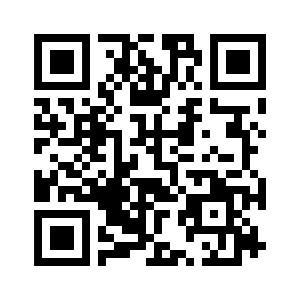
\includegraphics[width=0.5\textwidth]{github_repo.png}
    \end{imgbox}
\end{center}

\section*{Selbstständigkeitserklärung}

Hiermit bestätige ich, dass ich die vorliegende Maturaarbeit eigenständig angefertigt und dabei keine anderen als die angegeben Quellen und Hilfsmittel genutzt habe. Wörtliche oder inhaltliche Übernahmen aus fremden Werken oder Quellen sind ausnahmslos durch korrekte Zitate ausgewiesen.

\end{document}
% ENDE DOKUMENT -----------------------------------